%%%%%%%%%%%%%%%%%%%%%%%%%%%%%%%%%%%%%%%%%%%%%%%%%%%%%%%%%%%%%%%%%%%%%%%%%%%%%%%
% Chapter 2: Desarrollo
%%%%%%%%%%%%%%%%%%%%%%%%%%%%%%%%%%%%%%%%%%%%%%%%%%%%%%%%%%%%%%%%%%%%%%%%%%%%%%%

%++++++++++++++++++++++++++++++++++++++++++++++++++++++++++++++++++++++++++++++
En este capítulo dos se va a describir el desarrollo del proyecto. Se dividirá en dos fases bien diferenciadas, una primera fase que consiste en el análisis y refactorización del código fuente de la versión anterior de
{\it GitHub Education Shell}, y una segunda fase que trata de la incorporación de nuevas funcionalidades a la herramienta.
\bigskip

Por otro lado, también cabe nombrar la metodología de trabajo empleada. Situándonos en el marco de las metodologías ágiles, {\it Scrum} fue la metodología que mejor encajaba, teniendo en cuenta las características del proyecto.
Se ha optado por un desarrollo incremental, en lugar de una planificación y ejecución estricta de las tareas. Además, en numerosas ocasiones,
se produjeron solapamientos de las diferentes partes del desarrollo, en vez de un ciclo secuencial. También fueron frecuentes las reuniones con el tutor, en las que se comentaban tanto avances como dificultades.

%++++++++++++++++++++++++++++++++++++++++++++++++++++++++++++++++++++++++++++++

\section{Primera fase: análisis}
\label{2:sec:1}

En esta sección, se explicará detalladamente el proceso fundamental de la primera fase de este Trabajo de Fin de Grado.
\bigskip

El análisis del código fuente correspondiente a la primera versión de {\it ghedsh}, se ha llevado a cabo con la finalidad de identificar aquellas partes mejorables del diseño e implementación,
puesto que una de las prioridades era facilitar el desarrollo colaborativo y, para ello, se requiere que el código sea limpio y fácil de entender, lo más auto-explicativo posible.
\bigskip
%-------------------------------------------------------------------------------
\subsection{Estructura del repositorio}
\label{2.1.1}
En la figura \ref{fig:masterv1}, se muestra la estructura del repositorio de la primera versión de {\it ghedsh}, en concreto, de la rama \verb master. Dicha estructura corresponde con la forma estándar
de organizar el código de las gemas.

\begin{figure}[H]
\begin{center}
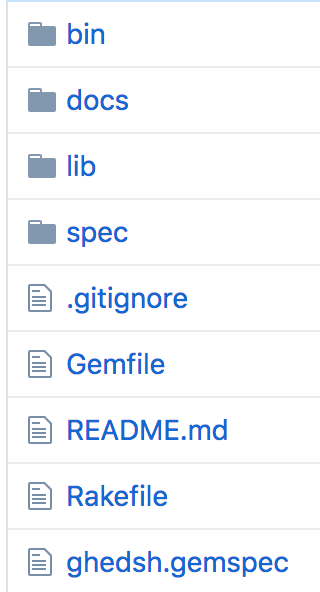
\includegraphics[width=0.20\textwidth]{images/estructura-inicial}
\caption{Estructura del repositorio (primera versión).}
\label{fig:masterv1}
\end{center}
\end{figure}

A continuación, se explicarán los componentes principales del repositorio:
\begin{itemize}
  \item {\it \textbf{bin}}: incluye el ejecutable de la gema, que se cargará en el \verb $PATH  del usuario.
  \item {\it \textbf{lib}}: en este directorio se encuentra el código fuente de la gema.
  \item {\it \textbf{spec}} o {\it \textbf{test}}: aquí se definirán las pruebas, que dependrán del {\it framework} de tests que utilice el desarrollador.
  \item {\it \textbf{Gemfile}}: es un fichero donde se especifican las dependencias del programa.
  \item {\it \textbf{Rakefile}}: se trata de un fichero muy común en las gemas. Su función es, principalmente, la automatización de tareas.
  \item {\it \textbf{gemspec}}: en este último fichero se incluye toda la información acerca de la gema, como, por ejemplo,
  su versión, plataforma soportada, versión de Ruby requerida y nombre y correo electrónico del autor o autores.
\end{itemize}
\bigskip
%----------------------------------------------------------------------
\subsection{Contenido del repositorio}
\label{2.1.2}
El primer paso del análisis consistió en comprender exactamente el flujo del programa. Ésto es necesario dado que, para identificar las partes mejorables del diseño inicial, requiere entenderlo en profundidad.
\bigskip

En la figura \ref{fig:lib}, vemos el contenido de \verb /lib :

\begin{figure}[H]
  \begin{center}
  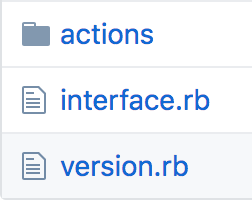
\includegraphics[width=0.25\textwidth]{images/lib}
  \caption{Contenido del directorio lib.}
  \label{fig:lib}
  \end{center}
\end{figure}

Los dos ficheros que ahí se encuentan son: \verb interface.rb  y \verb version.rb  .
\bigskip

En cuanto a \verb interface.rb , implementa la clase {\it Interface}. Ésta clase lleva a cabo el bucle principal característico de los CLI, se trata del bucle {\it Lectura-Evaluación-Impresión}
(en inglés, {\it REPL, Read-Eval-Print-Loop} \cite{B9}), que consiste en:
\begin{itemize}
  \item \textbf{Lectura}: parsea la entrada del usuario y determina si existe esa acción en la estructura de datos interna.
  \item \textbf{Evaluación}: una vez que se acepta la entrada del usuario se ejecutan las acciones con los parámetros especificados, si son necesarios. Es aquí donde se realiza el manejo de errores y excepciones.
  \item \textbf{Impresión}: muestra al usuario el resultado obtenido tras realizar el paso de evaluación.
\end{itemize}

Por otro lado, el fichero \verb version.rb , contiene una constante que indica la versión de la gema {\it ghedsh}. También cabe nombrar que, para asignar un identificador numérico a cada estado del software, se ha utilizado {\it Semantic Versioning} \cite{B10}.
\bigskip

A grandes rasgos, este esquema de control de versiones tiene la estructura {\it MAJOR.MINOR.PATCH}, donde
{\it MAJOR} se incrementa cuando se realizan cambios en la API que no son retrocompatibles. {\it MINOR} se modifica al añadir nuevas funcionalidades que sí son retrocompatibles y, por último, {\it PATCH} varía al corregir {\it bugs} en el software.
Un ejemplo de versión sería:
\begin{itemize}
  \item \verb ghedsh  \verb version  \verb 2.3.6 .
\end{itemize}
\bigskip

En cuanto al directorio \verb /lib/actions , la figura \ref{fig:actions} muestra el contenido del mismo:
\begin{figure}[H]
  \begin{center}
  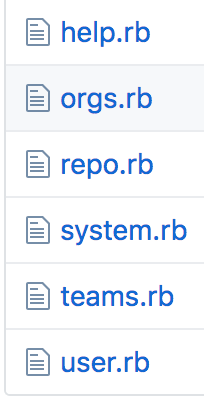
\includegraphics[width=0.17\textwidth]{images/actions}
  \caption{Contenido del directorio actions}
  \label{fig:actions}
  \end{center}
\end{figure}
\bigskip

Los ficheros principales se describirán según la funcionalidad que desempeñan:
\begin{itemize}
  \item \verb orgs.rb : proporciona los métodos necesarios relacionados con las organizaciones para comunicarse con la API de GitHub.
  \item \verb repo.rb : agrupa métodos que llevan a cabo tareas relacionadas con los repositorios, nuevamente, haciendo uso de la API de GitHub.
  \item \verb teams.rb : de manera similar a los anteriores ficheros, especializado en tareas de equipos.
  \item \verb user.rb : agrupa métodos relacionados con el usuario.
  \item \verb system.rb : este fichero se encarga de crear los directorios de configuración de {\it ghedsh}.
\end{itemize}
\bigskip
%--------------------------------------------------------------------------------------
\subsection{Code Smell}
\label{2.1.3}
Una vez analizado el planteamiento inicial, se han detectado una serie de debilidades en el diseño que han dado lugar a diversos {\it code smell} \cite{B11}.
Un {\it code smell} se define como cualquier característica del código fuente que, posiblemente, indica un problema más profundo. No son considerados como {\it bugs}, puesto que no impiden que un programa funcione de manera correcta.
\bigskip

No obstante, estos defectos de diseño pueden afectar al rendimiento del programa, aumentan la probabilidad de errores en el futuro e, incluso, ralentizar el desarrollo del programa y dificultar la extensibilidad del mismo.
\bigskip

Determinar qué es y lo que no es un {\it code smell} para un código fuente específico suele tener un componente de juicio subjetivo, dado que puede variar según el lenguaje de programación utilizado, el desarrollador y la metodología de desarrollo aplicada. Pero, por otro lado, valorar 
los posibles casos de uso, aporta indicaciones para respetar ciertos principios y calidad del software.
\bigskip

En el apartado de refactorización se explicará cómo se ha procedido para solucionarlos. A continuación, se expondrán los {\it code smells} más significativos encontrados en la primera versión de {\it ghedsh}. 
%--------------------------------------------------------------------------------------
  \subsubsection{{\it \textbf{Switch Statements}}}
  Suele ser muy característico de los códigos orientados a objetos. Esencialmente, el problema con las sentencias \verb switch-case  o sentencias \verb if  es la duplicación de código.
  Al utilizarlas con un conjunto de números o cadenas (normalmente, asignadas a constantes) que conforman una lista de valores permitidos para una entidad, existe una dependencia en ellas para decidir la entidad correcta a utilizar en cada momento.
  \bigskip

  Como consecuencia, al añadir nuevos casos, debemos localizar todas estas sentencias en el código y modificarlas.
  Para ilustrarlo con ejemplos, véase las figuras \ref{fig:constantes}, \ref{fig:switch-smell} y \ref{fig:switch-smell2}.
  \bigskip

  \begin{figure}[H]
    \begin{center}
    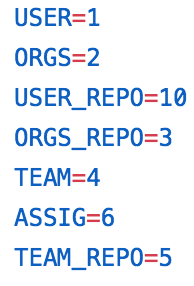
\includegraphics[width=0.18\textwidth]{images/constantes}
    \caption{Constantes numéricas que deciden la entidad a utilizar.}
    \label{fig:constantes}
    \end{center}
  \end{figure}

  \begin{figure}[H]
    \begin{center}
    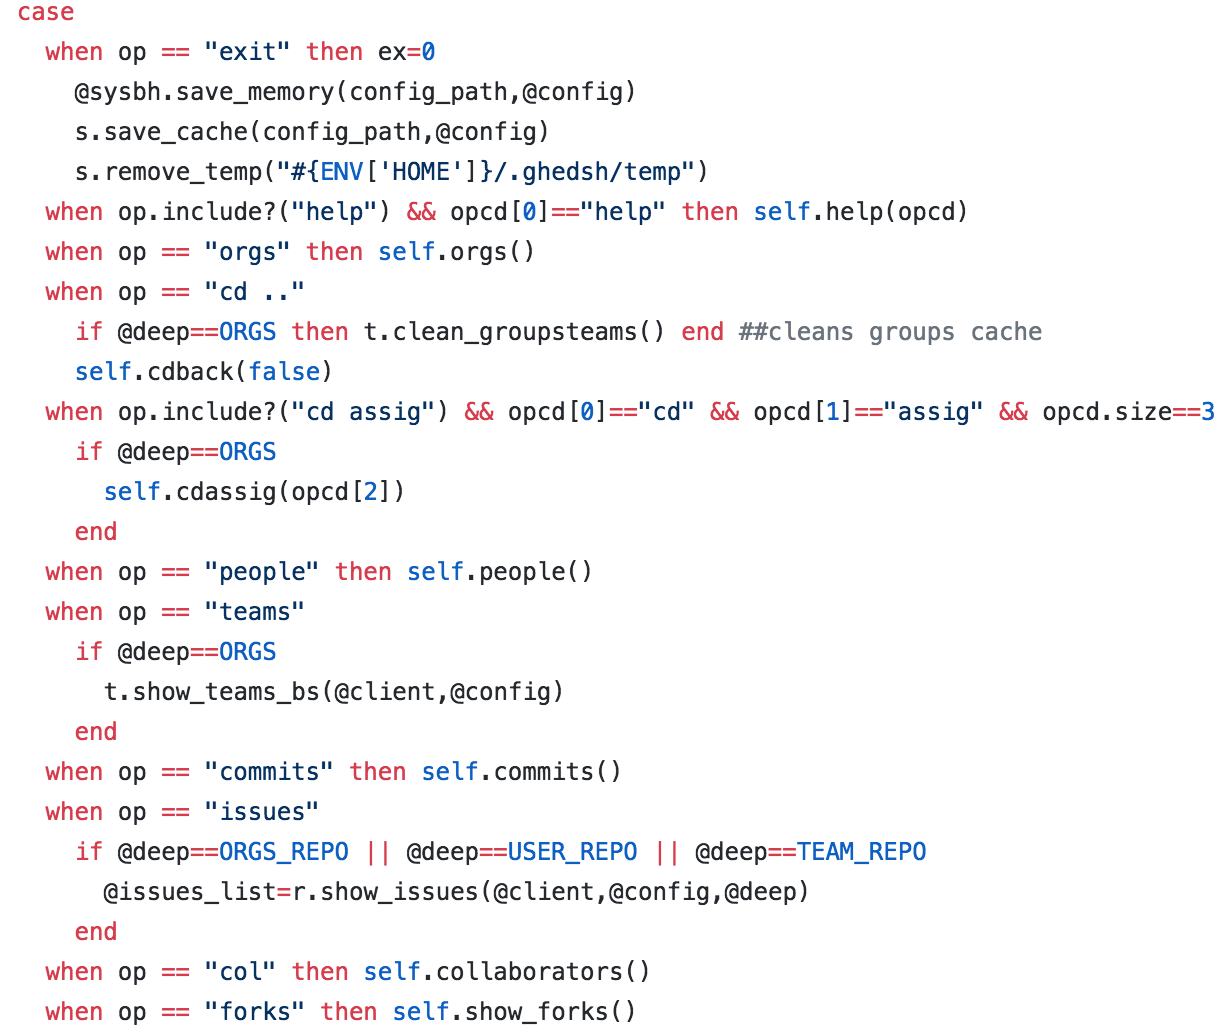
\includegraphics[width=0.89\textwidth]{images/switch-smell}
    \caption{Ejemplo de switch smell, en interface.rb.}
    \label{fig:switch-smell}
    \end{center}
  \end{figure}
  \bigskip

  \begin{figure}[H]
    \begin{center}
    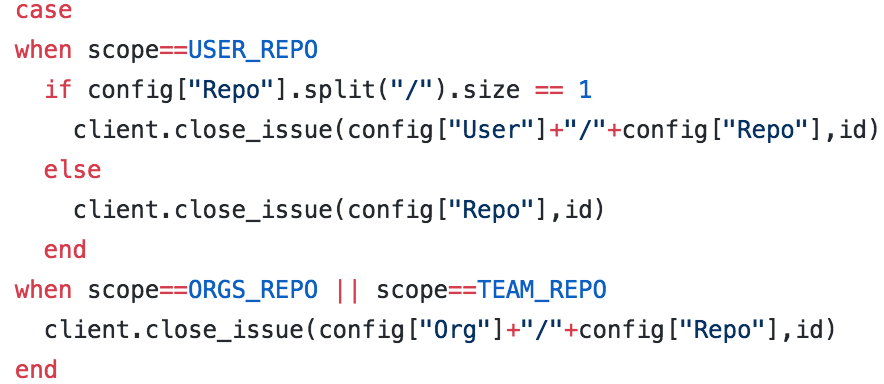
\includegraphics[width=0.70\textwidth]{images/switch-smell2}
    \caption{Otro caso de switch smell, en repo.rb.}
    \label{fig:switch-smell2}
    \end{center}
  \end{figure}
  \bigskip

  Este tipo de {\it smell} es el más repetido a lo largo del código de la primera versión de {\it ghedsh}, por lo que gran parte del proceso de refactorización se ha centrado en este aspecto.
  \bigskip
%-------------------------------------------------------------------------------------
  \subsubsection{{\it \textbf{Long Method}}} 
  Se trata de un {\it smell} que se clasifica a nivel de métodos. Como su nombre indica (método largo), consiste en un método que ha crecido demasiado. 
  \bigskip

  Escribir código suele ser más fácil que interpretarlo. Por ello, muchas veces este {\it smell} pasa desapercibido hasta que el método toma un tamaño considerable y dificulta saber qué es lo que realmente hace. Por esta razón,
  definir métodos más cortos con un nombre significativo, facilita la mantenibilidad del código y su lectura.
  \bigskip
%----------------------------------------------------------------------------
  \subsubsection{{\it \textbf{Large Class}}}
  {\it Large Class} se clasifica dentro de los {\it smells} a nivel de clases. Indica que una clase definida ha crecido excesivamente en tamaño ({\it God Object} \cite{B12}), es decir, realiza demasiadas cosas y que, seguramente, su funcionalidad puede descomponerse
  en clases más pequeñas y fáciles de manejar. Como suele ocurrir en los casos anteriormente nombrados, éste {\it smell} propicia también la duplicación de código.

%---------------------------------------------------------------------------------
\section{Segunda fase: refactorización}
\label{2:sec:2}

En este apartado, se explicará el proceso de refactorización efectuado en el código fuente de {\it ghedsh}. El principal objetivo es el cumplimiento del principio {\it Open/Closed} \cite{B13}, que pertenece a un grupo de cinco principios fundamentales (S.O.L.I.D \cite{CBle:2010}) de la programación orientada a objetos y cuya finalidad es
hacer los diseños de software más comprensibles, flexibles y mantenibles.
%-----------------------------------------------------------------------------------
\subsection{Principios de diseño S.O.L.I.D}
\label{2.2.1}
Se desarrollará ahora el significado de este acrónimo:
\begin{itemize}
  \item {\it \textbf{S}ingle Responsibility}: establece que una clase debería de tener sólo una responsabilidad, es decir, si fuera necesario modificar dicha clase, debe ser por un único motivo.
  \item {\it \textbf{O}pen/Closed}: una entidad software debería estar abierta para extensión y cerrada para modificación. En el siguiente párrafo se explicará con más detalle este principio.
  \item {\it \textbf{L}iskov Substitution}: los objetos de un programa deberían ser sustituíbles por subtipos de ese objeto, sin afectar al correcto funcionamiento de ese programa.
  \item {\it \textbf{I}nterface Segregation}: indica que es preferible muchas interfaces cliente específicas, en lugar de una interfaz de propósito general.
  \item {\it \textbf{D}ependency Inversion}: sugiere que se debe depender de abstracciones, no de implementaciones. Esto da lugar a la técnica inyección de dependencias.
\end{itemize}
\bigskip

Como se ha indicado anteriormente, se procederá a detallar el principio {\it Open/Closed}, puesto que es bastante necesario desde el punto de vista del desarrollo de {\it ghedsh}. La principal razón es que, si otro desarrollador desea incluir nuevas funcionalidades, no necesitaría alterar el código original de la gema.
\bigskip

Este principio establece que, las entidades de software, ya sean módulos, funciones, clases, etcétera, deberían estar abiertas para la extensión de su comportamiento, pero cerradas para su modificación. Ésto se consigue, por ejemplo, mediante herencia, reescribiendo los métodos de la clase madre, pudiendo incluso ser abstracta dicha clase.
Otra manera sería por medio de inyección de dependencias, que tienen la misma interfaz pero distinto funcionamiento.

%---------------------------------------------------------------------------------
\subsection{Refactorización: Strategy pattern}
\label{2.2.2}
En esta sección se expondrá el proceso que se ha seguido para eliminar el {\it switch smell}. El proceso ha consistido, fundamentalmente,
en la aplicación del patrón estrategia (en inglés, {\it Strategy pattern} \cite{jspatterns:2012}).
\bigskip

{\it Strategy} es un patrón que permite a un programa seleccionar un algoritmo particular en tiempo de ejecución. El propósito de este patrón es proporcionar una manera clara 
de definir familias de algoritmos, encapsulando cada uno como objeto para poder intercambiarlos fácilmente. El principal beneficio de este modelo es que el objeto cliente puede elegir aquel algoritmo que le conviene y
permutarlo dinámicamente según sus necesidades.
\bigskip

En cuanto a cómo se ha aplicado este patrón, primero ha sido necesario modificar el diseño inicial propuesto en la primera versión de {\it ghedsh}.
De manera que, en el directorio \verb /lib \verb /actions , se han reescrito las clases que allí se encontraban y su propósito también ha cambiado, dado que ya no se agrupan métodos para repositorios, organizaciones, equipos, etcétera, sino que
contendrán las acciones permitidas en cada uno de estos contextos. De este modo, aunque las acciones sean permitidas en varios contextos, cada clase conocerá su propia implementación.
\bigskip

A partir de la segunda versión, en \verb /lib \verb /actions , se encuentran las siguientes clases:
\begin{itemize}
  \item \verb orgs.rb : se define la clase \verb Organization , contiene los métodos de las acciones permitidas para las organizaciones.
  \item \verb system.rb : contiene la clase que se encarga de gestionar los directorios de configuración de {\it ghedsh}, así como guardar la configuración del usuario.
  \item \verb teams.rb : se define la clase \verb Team , que incluye los métodos de las acciones permitidas para los equipos.
  \item \verb user.rb : incluye en la clase \verb User , los métodos correspondientes a las acciones que se permiten en el contexto de usuario.
\end{itemize}
\bigskip

Por otro lado, en \verb /lib/interface.rb  (véase la figura \ref{fig:new-loop}) se tiene un claro ejemplo de patrón estrategia, que se aplica en el bucle Lectura-Evaluación-Impresión (REPL). Esto permite decidir en tiempo de ejecución el comando que el usuario quiere utilizar.
Se parsea lo que ha introducido, de manera que el primer {\it token}, se refiere al nombre del comando deseado. Después, se busca dicho comando en la estructura de datos interna, en este caso, un {\it hash}, que consiste en una colección clave-valor en la que
la clave es el nombre que identifica el comando y el valor es la función que exporta la clase \verb Commands ,   la cual decide si es posible ejecutarlo, verificando si contexto actual responde a la acción solicitada por el usuario.
\begin{figure}[H]
  \begin{center}
  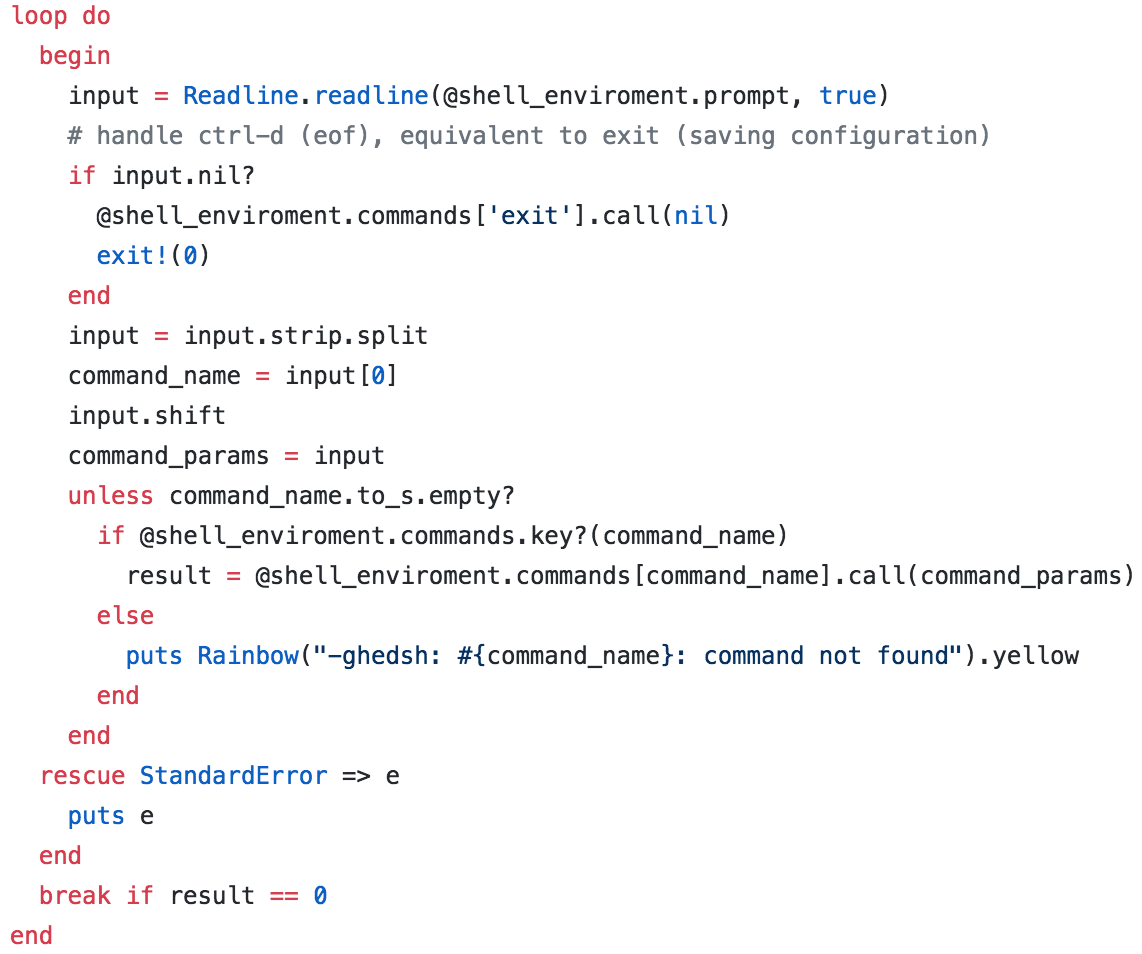
\includegraphics[width=0.80\textwidth]{images/new-loop}
  \caption{Bucle Lectura-Evaluación-Impresión sin sentencia switch/case.}
  \label{fig:new-loop}
  \end{center}
\end{figure}
\bigskip

Cabe destacar que, la figura \ref{fig:switch-smell} anteriormente indicada, representa una porción del código, puesto que ahí se encontraban {\it hard-coded} \cite{B15} todos los comandos.
Sin embargo, en la figura \ref{fig:new-loop} se encuentra todo el código del REPL, tarea en la que se especializa la clase \verb Interface .
\bigskip

Aparte, con este nuevo esquema se logra eliminar las constantes que deciden el tipo de clase a utilizar en cada momento (véase \ref{fig:constantes}), ya que, en esta segunda versión,
existe una variable que almacena el contexto y referencia directamente la clase con la que se realizan las acciones y ya no es necesario hacer la distinción entre, por ejemplo, repositorio de usuario, repositorio de organización y repositorio de equipo. Esto es así porque cada clase gestiona su contexto.
\bigskip
%----------------------------------------------------------------------------------------
\subsection{Refactorización: Extract Method}
\label{2.2.3}

Como resultado de aplicar el patrón {\it Strategy} y la reescritura de las clases encargadas de las acciones, también se ha solucionado el {\it Long Method smell}. Ésto se ha logrado reduciendo el cuerpo de la función, a través de la extracción de partes del código que realizan tareas similares,
dando lugar a nuevas funciones.
\bigskip

Para ilustrarlo mejor, en la siguiente porción de código vemos un ejemplo de {\it Extract Method} \cite{Fowler:1999} muy simple:
\bigskip 

\begin{minipage}[t]{0.45\linewidth}
  Problema:
  \begin{lstlisting}[language=Ruby]
    def print_owing(amount)
      print_banner

      # print details
      puts "name: #{@name}"
      puts "amount: #{amount}"
    end
  \end{lstlisting}
\end{minipage}
  %
\begin{minipage}[t]{0.5\linewidth}
    Solución (Extract Method):
  \begin{lstlisting}[language=Ruby]
    def print_owing(amount)
      print_banner
      print_details(amount)
    end

    def print_details(amount)
      puts "name: #{@name}"
      puts "amount: #{amount}"
    end
  \end{lstlisting}
\end{minipage}
\bigskip

Si llevamos esta idea a un programa real, los beneficios son claros:
\begin{itemize}
  \item Código más legible. Hay que destacar que, el nuevo método creado, debe llevar un nombre representativo, es decir, un nombre que describa su propósito.
  \item Menos duplicación de código. Muchas veces, el código contenido en una función puede ser reutilizado en otras partes del programa. Por lo tanto, reemplazamos el código repetido por llamadas al nuevo método.
  \item Mejor detección de errores. Al aislar partes de código, detectar dónde se ha producido un error es más fácil, hay son menos líneas que revisar.
\end{itemize}

%------------------------------------------------------------------------------------------------
\subsection{Refactorización: Extract Class}
\label{2.2.4}

El método de refactorización {\it Extract Class}\cite{Fowler:1999} ayudará a mantener la adherencia al principio {\it Single Responsibility} (SRP), comentado en la sección \ref{2.2.1}.
\bigskip

A menudo, las clases comienzan siendo claras, fáciles de entender y sólo tienen una única responsabilidad. Sin embargo, en algún punto, la clase empieza a crecer: se realizan nuevas operaciones, se añaden más datos y se incorporan nuevos métodos.
Por lo tanto, tarde o temprano esta clase acabe teniendo más de una responsabilidad.
\bigskip

A continuación, se explicarán una serie de pasos genéricos que guían a la hora de aplicar esta técnica:
\begin{itemize}
  \item \textbf{Paso 1}. Determinar qué se va a extraer. Tratar de buscar unidades lógicas de datos que actúan sobre un subconjunto de los datos.
  \item \textbf{Paso 2}. Crear una nueva clase. Las operaciones extraídas dan lugar a una nueva clase, que tiene que establecer un enlace (puede ser bidireccional) con la antigua clase.
  \item \textbf{Paso 3}. Renombrar la antigua clase. Si, tras la extracción, el nombre de la antigua clase carece de sentido, debemos renombrarla.
\end{itemize}

{\it Extract Class} se aplica mejor si hay unidades de datos que se agrupan según el contenido que almacenan o si hay operaciones que sólo se realizan en un subconjunto de los datos. Esto último ocurría en el código de la primera versión de {\it ghedsh}, ya que
la clase \verb Interface , se ocupaba de varias tareas, y una de ellas era gestionar el contexto del CLI.
\bigskip

Una vez que se determinó qué se iba a extraer, fue posible crear una clase nueva, \verb ShellContext , especializada únicamente en gestionar el entorno de {\it ghedsh}. Si éste se ha cargado correctamente,
\verb ShellContext   lo comparte con \verb Interface . Entonces, le permite saber cuáles son los comandos que están definidos, ejecutarlos y disponer de la configuración del usuario en cada momento.
\bigskip

Finalmente, el resultado es que la clase \verb Interface , se encarga exclusivamente de realizar el REPL con los datos que le proporciona el entorno (\verb ShellContext ). Por lo tanto, si se eliminasen los comandos definidos, el REPL se llevaría a cabo correctamente, con la diferencia de que no se ejecutaría ninguna acción.






